\documentclass{standalone}
\usepackage{tikz}
\usetikzlibrary{patterns, positioning}

\begin{document}
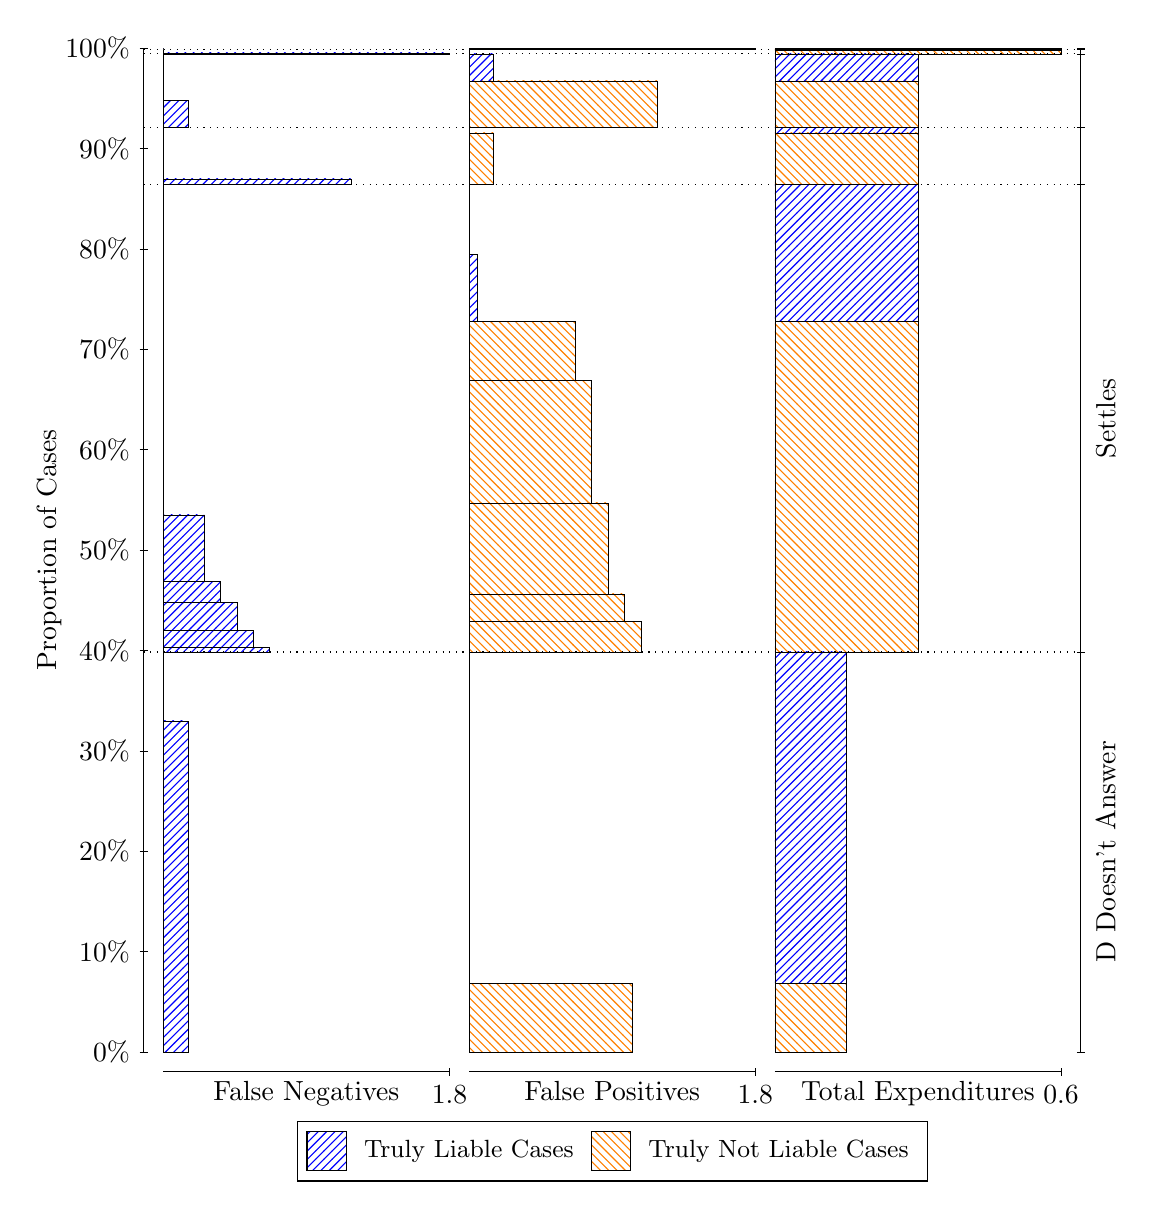
\begin{tikzpicture}
\draw[black, very thin] (1.5,1.75) -- (1.5,14.5);
\node[rotate=90, anchor=center] at (0.3, 8.125) {Proportion of Cases};
\draw[black, very thin] (1.45,1.75) -- (1.55,1.75);
\node[anchor=east] at (1.45, 1.75) {0\%};
\draw[black, very thin] (1.45,3.025) -- (1.55,3.025);
\node[anchor=east] at (1.45, 3.025) {10\%};
\draw[black, very thin] (1.45,4.3) -- (1.55,4.3);
\node[anchor=east] at (1.45, 4.3) {20\%};
\draw[black, very thin] (1.45,5.575) -- (1.55,5.575);
\node[anchor=east] at (1.45, 5.575) {30\%};
\draw[black, very thin] (1.45,6.85) -- (1.55,6.85);
\node[anchor=east] at (1.45, 6.85) {40\%};
\draw[black, very thin] (1.45,8.125) -- (1.55,8.125);
\node[anchor=east] at (1.45, 8.125) {50\%};
\draw[black, very thin] (1.45,9.4) -- (1.55,9.4);
\node[anchor=east] at (1.45, 9.4) {60\%};
\draw[black, very thin] (1.45,10.675) -- (1.55,10.675);
\node[anchor=east] at (1.45, 10.675) {70\%};
\draw[black, very thin] (1.45,11.95) -- (1.55,11.95);
\node[anchor=east] at (1.45, 11.95) {80\%};
\draw[black, very thin] (1.45,13.225) -- (1.55,13.225);
\node[anchor=east] at (1.45, 13.225) {90\%};
\draw[black, very thin] (1.45,14.5) -- (1.55,14.5);
\node[anchor=east] at (1.45, 14.5) {100\%};

\draw[black, very thin] (13.4,1.75) -- (13.4,14.5);
\draw[black, very thin] (13.35,1.75) -- (13.45,1.75);
\node[anchor=west] at (13.35, 1.75) {};
\draw[black, very thin] (13.35,6.8302) -- (13.45,6.8302);
\node[anchor=west] at (13.35, 6.8302) {};
\draw[black, very thin] (13.35,12.769) -- (13.45,12.769);
\node[anchor=west] at (13.35, 12.769) {};
\draw[black, very thin] (13.35,13.491) -- (13.45,13.491);
\node[anchor=west] at (13.35, 13.491) {};
\draw[black, very thin] (13.35,14.426) -- (13.45,14.426);
\node[anchor=west] at (13.35, 14.426) {};
\draw[black, very thin] (13.35,14.482) -- (13.45,14.482);
\node[anchor=west] at (13.35, 14.482) {};
\draw[black, very thin] (13.35,14.5) -- (13.45,14.5);
\node[anchor=west] at (13.35, 14.5) {};

\draw[black, very thin, pattern color=blue, pattern=north east lines] (1.75,1.75) rectangle (2.0614,5.9558);
\draw[black, very thin, pattern color=orange, pattern=north west lines] (1.75,5.9558) rectangle (1.75,6.8302);
\draw[black, very thin, pattern color=blue, pattern=north east lines] (1.75,6.8302) rectangle (3.0995,6.8907);
\draw[black, very thin, pattern color=blue, pattern=north east lines] (1.75,6.8907) rectangle (2.8919,7.0992);
\draw[black, very thin, pattern color=blue, pattern=north east lines] (1.75,7.0992) rectangle (2.6843,7.4561);
\draw[black, very thin, pattern color=blue, pattern=north east lines] (1.75,7.4561) rectangle (2.4767,7.7219);
\draw[black, very thin, pattern color=blue, pattern=north east lines] (1.75,7.7219) rectangle (2.269,8.5707);
\draw[black, very thin, pattern color=orange, pattern=north west lines] (1.75,8.5707) rectangle (1.75,12.769);
\draw[black, very thin, pattern color=blue, pattern=north east lines] (1.75,12.769) rectangle (4.1376,12.837);
\draw[black, very thin, pattern color=orange, pattern=north west lines] (1.75,12.837) rectangle (1.75,13.491);
\draw[black, very thin, pattern color=blue, pattern=north east lines] (1.75,13.491) rectangle (2.0614,13.833);
\draw[black, very thin, pattern color=orange, pattern=north west lines] (1.75,13.833) rectangle (1.75,14.426);
\draw[black, very thin, pattern color=blue, pattern=north east lines] (1.75,14.426) rectangle (5.3833,14.437);
\draw[black, very thin, pattern color=orange, pattern=north west lines] (1.75,14.437) rectangle (1.75,14.482);
\draw[black, very thin, pattern color=orange, pattern=north west lines] (1.75,14.482) rectangle (1.75,14.492);
\draw[black, very thin, pattern color=blue, pattern=north east lines] (1.75,14.492) rectangle (1.75,14.5);
\draw[black, very thin, pattern color=orange, pattern=north west lines] (5.6333,1.75) rectangle (7.7095,2.6244);
\draw[black, very thin, pattern color=blue, pattern=north east lines] (5.6333,2.6244) rectangle (5.6333,6.8302);
\draw[black, very thin, pattern color=orange, pattern=north west lines] (5.6333,6.8302) rectangle (7.8133,7.2226);
\draw[black, very thin, pattern color=orange, pattern=north west lines] (5.6333,7.2226) rectangle (7.6057,7.5686);
\draw[black, very thin, pattern color=orange, pattern=north west lines] (5.6333,7.5686) rectangle (7.3981,8.7235);
\draw[black, very thin, pattern color=orange, pattern=north west lines] (5.6333,8.7235) rectangle (7.1905,10.283);
\draw[black, very thin, pattern color=orange, pattern=north west lines] (5.6333,10.283) rectangle (6.9829,11.028);
\draw[black, very thin, pattern color=blue, pattern=north east lines] (5.6333,11.028) rectangle (5.7371,11.877);
\draw[black, very thin, pattern color=blue, pattern=north east lines] (5.6333,11.877) rectangle (5.6333,12.769);
\draw[black, very thin, pattern color=orange, pattern=north west lines] (5.6333,12.769) rectangle (5.9448,13.423);
\draw[black, very thin, pattern color=blue, pattern=north east lines] (5.6333,13.423) rectangle (5.6333,13.491);
\draw[black, very thin, pattern color=orange, pattern=north west lines] (5.6333,13.491) rectangle (8.021,14.084);
\draw[black, very thin, pattern color=blue, pattern=north east lines] (5.6333,14.084) rectangle (5.9448,14.426);
\draw[black, very thin, pattern color=orange, pattern=north west lines] (5.6333,14.426) rectangle (5.6333,14.472);
\draw[black, very thin, pattern color=blue, pattern=north east lines] (5.6333,14.472) rectangle (5.6333,14.482);
\draw[black, very thin, pattern color=orange, pattern=north west lines] (5.6333,14.482) rectangle (9.2667,14.492);
\draw[black, very thin, pattern color=blue, pattern=north east lines] (5.6333,14.492) rectangle (7.1905,14.5);
\draw[black, very thin, pattern color=orange, pattern=north west lines] (9.5167,1.75) rectangle (10.425,2.6244);
\draw[black, very thin, pattern color=blue, pattern=north east lines] (9.5167,2.6244) rectangle (10.425,6.8302);
\draw[black, very thin, pattern color=orange, pattern=north west lines] (9.5167,6.8302) rectangle (11.333,11.028);
\draw[black, very thin, pattern color=blue, pattern=north east lines] (9.5167,11.028) rectangle (11.333,12.769);
\draw[black, very thin, pattern color=orange, pattern=north west lines] (9.5167,12.769) rectangle (11.333,13.423);
\draw[black, very thin, pattern color=blue, pattern=north east lines] (9.5167,13.423) rectangle (11.333,13.491);
\draw[black, very thin, pattern color=orange, pattern=north west lines] (9.5167,13.491) rectangle (11.333,14.084);
\draw[black, very thin, pattern color=blue, pattern=north east lines] (9.5167,14.084) rectangle (11.333,14.426);
\draw[black, very thin, pattern color=orange, pattern=north west lines] (9.5167,14.426) rectangle (13.15,14.472);
\draw[black, very thin, pattern color=blue, pattern=north east lines] (9.5167,14.472) rectangle (13.15,14.482);
\draw[black, very thin, pattern color=orange, pattern=north west lines] (9.5167,14.482) rectangle (13.15,14.492);
\draw[black, very thin, pattern color=blue, pattern=north east lines] (9.5167,14.492) rectangle (13.15,14.5);
\draw[black, dotted] (1.5,6.8302) -- (13.4,6.8302);
\draw[black, dotted] (1.5,12.769) -- (13.4,12.769);
\draw[black, dotted] (1.5,13.491) -- (13.4,13.491);
\draw[black, dotted] (1.5,14.426) -- (13.4,14.426);
\draw[black, dotted] (1.5,14.482) -- (13.4,14.482);
\draw[black, very thin] (1.75,1.5) -- (5.3833,1.5);
\node[anchor=north] at (3.5667, 1.5) {False Negatives};
\draw[black, very thin] (5.3833,1.45) -- (5.3833,1.55);
\node[anchor=north] at (5.3833, 1.45) {1.8};

\draw[black, very thin] (5.6333,1.5) -- (9.2667,1.5);
\node[anchor=north] at (7.45, 1.5) {False Positives};
\draw[black, very thin] (9.2667,1.45) -- (9.2667,1.55);
\node[anchor=north] at (9.2667, 1.45) {1.8};

\draw[black, very thin] (9.5167,1.5) -- (13.15,1.5);
\node[anchor=north] at (11.333, 1.5) {Total Expenditures};
\draw[black, very thin] (13.15,1.45) -- (13.15,1.55);
\node[anchor=north] at (13.15, 1.45) {0.6};

\node[black, centered, rotate=90] at (13.72, 4.2901) {D Doesn't Answer};
\node[black, centered, rotate=90] at (13.72, 9.7995) {Settles};





\draw (7.449999999999999,1.5) node[draw=none] (baseCoordinate) {};
\begin{scope}[align=center]
        \matrix[scale=0.5, draw=black, below=0.5cm of baseCoordinate, nodes={draw}, column sep=0.1cm]{
            \node[rectangle, draw, minimum width=0.5cm, minimum height=0.5cm, pattern=north east lines, pattern color=blue] {}; &
            \node[draw=none, font=\small] (B) {Truly Liable Cases}; &
            \node[rectangle, draw, minimum width=0.5cm, minimum height=0.5cm, pattern=north west lines, pattern color=orange] {}; &
            \node[draw=none, font=\small] (B) {Truly Not Liable Cases}; \\
            };
\end{scope}

\end{tikzpicture}
\end{document}